%% ---------------------------------------------------------------------------
%% IEEE conference paper (at most six pages) — architecture and operation of
%% the system. Written in plain language for a non-specialist reader.
%% Built with the official IEEEtran class (v1.8b), bundled in this directory.
%%
%% The figures are drawn with Graphviz and Mermaid; their sources and the
%% script that renders them to vector PDF live in diagrams/:
%%
%%   cd diagrams && ..\..\..\.venv\Scripts\python.exe render_diagrams.py
%%
%% Compile:  pdflatex paper.tex   (run twice, so cross-references resolve)
%% ---------------------------------------------------------------------------
\documentclass[conference]{IEEEtran}

\usepackage[T1]{fontenc}
\usepackage[utf8]{inputenc}
\usepackage{amsmath}
\usepackage{booktabs}
\usepackage{graphicx}
\usepackage{microtype}
\usepackage{xcolor}

\definecolor{linkblue}{HTML}{1F4E79}

\usepackage[colorlinks=true,allcolors=linkblue,breaklinks=true]{hyperref}
\usepackage{url}

\graphicspath{{figures/}}
\hyphenation{ac-cre-di-ta-tion re-triev-al doc-u-ment work-sta-tion}

\begin{document}

\title{Grounded Local AI for University Accreditation}

\author{\IEEEauthorblockN{Alfa Yohannis}
\IEEEauthorblockA{\textit{Faculty of Science and Technology} \\
\textit{Pradita University}, Tangerang, Indonesia \\
alfa.ryano@pradita.ac.id}}

\maketitle

\begin{abstract}
Preparing a university accreditation submission means answering hundreds of
detailed questions, and the evidence for each is buried somewhere in a shared
folder of thousands of files. This paper describes a working system that lets
staff ask a question in everyday Indonesian and receive an answer in seconds, in
which every statement carries a numbered citation pointing to the exact file and
page, sheet or slide it came from. It is built on retrieval-augmented
generation: the institution's own documents are searched first---by meaning and
by exact wording, with the two rankings fused and re-scored---and the language
model may write only from what was found. We describe the architecture, the
indexing and answering pipelines, and the engineering that makes the answers
checkable and the system dependable: source files are never modified, an index
of 1{,}497 files rebuilds incrementally while colleagues keep editing the drive,
answers survive dropped connections, and the whole system runs on one office
workstation with an 8\,GB graphics card, so confidential material need not
leave the building.
\end{abstract}

\begin{IEEEkeywords}
retrieval-augmented generation, document question answering, accreditation,
hybrid retrieval, large language models, higher education
\end{IEEEkeywords}

%% ===========================================================================
\section{Introduction}

An accreditation submission is an exercise in evidence. For every claim a study
programme makes---about its curriculum, its lecturers, its graduates, its
research---an assessor may ask where the proof is. The proof exists: in a decree
issued three years ago, in row~47 of a spreadsheet, on page~12 of a curriculum
document. It is simply spread across thousands of files accumulated over years
in a shared drive that several colleagues edit at once.

The consequence is familiar: a single question can cost half an hour of opening
files one by one, and under deadline pressure the tempting shortcut is to answer
from memory---which is how an unsupported claim reaches an assessor. A
general-purpose chatbot does not help. It has never seen these documents, yet it
still produces a fluent answer, and a fluent answer that cites nothing is
exactly the failure, known as hallucination~\cite{ji}, that an audited process
cannot tolerate. What is needed is a system that answers \emph{only} from the
institution's own files, and shows its working.

This paper reports such a system, built for and used in the accreditation of a
Master's programme in informatics under the Indonesian independent accreditation
agency for informatics and computing (LAM~INFOKOM). Its contribution is not a
new algorithm but a complete, deployed design, and the reasoning behind it:
\begin{itemize}
\item an architecture (Section~\ref{sec:architecture}) that answers with
  page-level citations while running entirely on one desktop computer;
\item an indexing pipeline (Section~\ref{sec:indexing}) that keeps the location
  of every passage and tolerates a shared drive that changes while it reads;
\item an answering pipeline (Section~\ref{sec:answering}) that combines search
  by meaning with search by exact wording, because accreditation documents need
  both;
\item the engineering that makes the system safe to point at a live archive and
  usable on a phone (Sections~\ref{sec:delivery}--\ref{sec:workstation}), and a
  frank account of its limits (Section~\ref{sec:limits}).
\end{itemize}

%% ===========================================================================
\section{Background}

\emph{Retrieval-augmented generation} (RAG) pairs a language model with a search
step: passages relevant to the question are retrieved from a document
collection and placed in the model's input, so that the answer can draw on them
rather than on what the model memorised in training~\cite{lewis,gaosurvey}.
Grounding the answer this way reduces, though does not eliminate, invented
content; asking the model to cite the passage behind each statement makes the
remaining errors visible to the reader~\cite{alce}.

How well RAG works depends first on the search. Classical keyword ranking such
as BM25~\cite{bm25} matches the words of the question and excels at names and
identifiers. Dense retrieval represents question and passage as vectors from a
neural encoder and matches them by meaning~\cite{dpr}, catching paraphrases that
share no words. Neither dominates: on a broad benchmark, BM25 remains a strong
baseline that many dense models fail to beat outside the data they were trained
on~\cite{beir}. Results from several rankers can be merged by reciprocal rank
fusion~\cite{rrf}, and a cross-encoder, which reads question and passage
together, can then re-score the merged shortlist more accurately than either
first-stage method~\cite{nogueira}. Finally, more context is not always better:
language models make less use of material in the middle of a long
input~\cite{liu}, which argues for passing the model a few good passages rather
than many mediocre ones.

The system described here assembles these established pieces under the
constraints of its setting: an audited purpose, a confidential and constantly
edited archive, Indonesian documents mixing prose with decree numbers, and
modest hardware.

%% ===========================================================================
\section{Requirements and User View}

Five requirements, all taken from the accreditation setting, shaped the design:
\begin{enumerate}
\item[R1] \emph{Checkable}: every statement must lead, in one click, to the
  file and the page, sheet or slide that supports it.
\item[R2] \emph{Hands off the archive}: nothing may ever modify the drive.
\item[R3] \emph{Private by default}: documents stay in the building.
\item[R4] \emph{Modest hardware}: one desktop with a consumer graphics card.
\item[R5] \emph{Dependable in daily use}: colleagues edit the drive while it is
  indexed, and users ask from phones on unreliable Wi-Fi.
\end{enumerate}

The system is a web page that opens in any browser on the office network,
offering a single box for a question in Indonesian. Seconds later an answer
appears in ordinary prose, a small numbered marker beside each statement, and
beside it an evidence panel: one card per marker giving the document's name, the
page or sheet the passage came from, and the passage itself. Clicking a card
opens or downloads the original file. The user is therefore never asked to
trust the system---every sentence can be checked in one click (R1).

Asked whether the programme teaches machine learning, for instance, the system
replies that the curriculum lists a \emph{Machine Learning and Deep Learning}
course, and attaches the curriculum spreadsheet and the sheet its course table
sits on, so the reader can open it and see the row. Questions can be limited to
one criterion's folder, and every exchange is kept in a saved conversation.

%% ===========================================================================
\section{Architecture}
\label{sec:architecture}

\begin{figure*}[t]
\centering
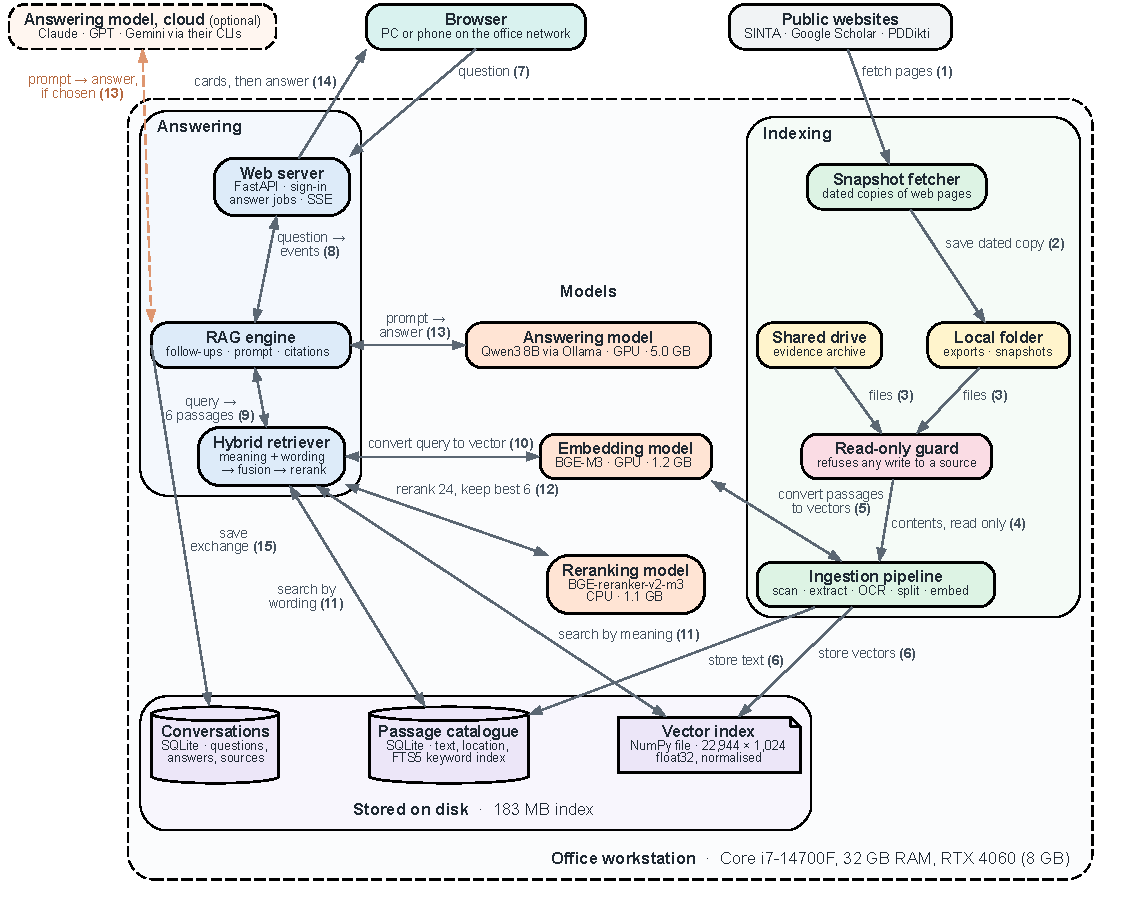
\includegraphics[width=\textwidth]{architecture}
\caption{System architecture. Everything inside the dashed boundary runs on one
office workstation. Colours mark roles---sources (yellow), the read-only guard
(rose), indexing (green), models (peach), serving (blue), stored data
(lavender), people's devices (mint) and outside services (grey). Arrows are
numbered by step, as explained in Section~\ref{sec:architecture}; two-headed
arrows are calls that return a result. The dashed arrow to a cloud model is the
only path by which document text can leave the building.}
\label{fig:arch}
\end{figure*}

Fig.~\ref{fig:arch} shows the system's parts. It is easiest to read as two
activities that never run into each other and meet only at the stored index;
the step numbers in this section refer to its arrows.

\emph{Indexing} (right of the figure, steps 1--6) turns the archive into
something searchable. Public web pages are fetched (step~1) and saved as dated
copies in a local folder (step~2), beside exports copied out of the shared
drive. Files from both folders reach the ingestion pipeline only through the
read-only guard (steps 3--4). The pipeline splits every document into passages,
has the embedding model turn each passage into a vector (step~5), and stores
every passage twice (step~6): as text in a SQLite database with a full-text
keyword index, and as a vector in a NumPy matrix. Section~\ref{sec:indexing}
follows this path in detail.

\emph{Answering} (left, steps 7--15) serves one question at a time. The browser
sends the question (step~7) to a web server built with FastAPI, which handles
sign-in and starts an \emph{answer job}: the job hands the question to the RAG
engine and relays the events it produces (step~8). The engine asks the hybrid
retriever for passages (step~9). The retriever has the embedding model turn the
question into a vector (step~10), searches the index by meaning and by wording
for 40 passages each (step~11), and has the reranking model keep the best six
of the 24 that survive fusion (step~12). The engine then sends a prompt built
from those six passages to the answering model---local by default, or a cloud
model if the user chose one---and receives the answer (step~13). The server
streams the evidence cards and then the answer to the browser (step~14), and
the engine saves the exchange in the conversation store (step~15).
Section~\ref{sec:answering} follows this path in detail.

The embedding model is BGE-M3~\cite{bge}, a multilingual model that handles
Indonesian well and produces vectors of 1{,}024 numbers; the reranking model is
a cross-encoder from the same family; and the answering model is, by default,
Qwen3 with 8 billion parameters~\cite{qwen}, served on the same machine by
Ollama (Table~\ref{tab:models}).

The code is Python, with dependencies running one way: the storage layer knows
nothing about the web, and the web server never touches the database directly.
The browser interface is plain JavaScript with no build step. An administrator
account may also re-index; a guest account may only ask, and the server itself
refuses indexing requests from it. Passwords are stored as salted PBKDF2 hashes
and sessions as HMAC-signed cookies.

%% ===========================================================================
\section{Indexing Pipeline}
\label{sec:indexing}

\begin{figure}[t]
\centering
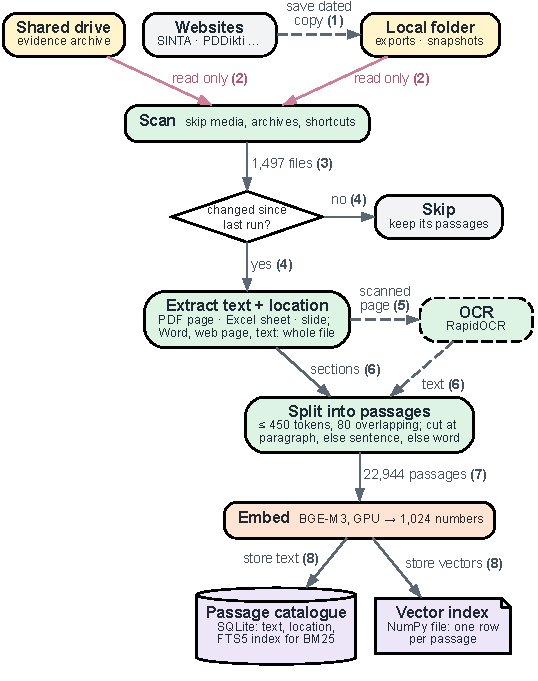
\includegraphics[width=\columnwidth]{ingestion}
\caption{Indexing pipeline, with steps numbered as explained in
Section~\ref{sec:indexing}. Dashed steps run only when needed.}
\label{fig:ingest}
\end{figure}

Fig.~\ref{fig:ingest} shows the steps every file goes through, in order; the
step numbers in this section refer to its arrows.

\subsubsection{Scan and change detection}
The scanner walks both folders through the read-only guard (step~2), skipping
media, archives, executables and Google Drive shortcut files, which contain no
text, and any file over 200\,MB. For each of the 1{,}497 remaining files
(step~3) it records a signature made of the file's size and last modification
time. If the signature matches the one stored from the previous run, the file
is skipped and its passages are kept; otherwise it goes on to extraction
(step~4). Detecting change this way
costs one directory listing rather than reading every file, so a daily update
finishes in seconds instead of the tens of minutes a full pass takes---almost
all of it spent computing vectors.

\subsubsection{Extraction that remembers where text was}
Each format has its own extractor, and each produces \emph{labelled sections}
rather than one block of text: a PDF yields one section per page, a workbook one
per sheet, a slide deck one per slide, while Word documents, web pages and text
files form a single section. Word tables are flattened row by row with column
separators, and spreadsheet rows keep their cells tab-separated, so tabular
structure survives into the text the model sees. These labels are what make a
citation such as ``page~12'' or ``sheet \emph{Dosen}'' possible later.
Table~\ref{tab:corpus} shows the result for the deployed archive.

A PDF page yielding fewer than 60 characters is almost certainly a scan of a
signed decree or certificate. Such pages are counted, and passed to optical
character recognition (step~5; OCR, RapidOCR at 200\,dpi, at most 80 pages per
document). The extracted sections and the recognised text then go on to be
split (step~6); passages recovered by OCR are marked, and the model is told to
add a caution when it quotes a number from one.

Evidence on public websites---the national research index SINTA, Google Scholar
profiles, the higher-education database PDDikti and staff pages on the
university site---is fetched by a separate snapshot run and saved as dated text
in the local folder (step~1), which is then indexed like any other document. Each snapshot records its
address and retrieval time, and repeats that marker throughout its text, so
that a passage cut from the middle of a long page still says where it came
from.

\begin{table}[t]
\caption{The deployed archive, by file type}
\label{tab:corpus}
\centering
\footnotesize
\begin{tabular}{@{}lrrrl@{}}
\toprule
Type & Files & With text & Passages & Cited as \\
\midrule
PDF                      & 894 & 760 & 16{,}923 & page $n$ \\
Word                     & 173 & 170 &  3{,}616 & whole document \\
Excel                    &  55 &  55 &  1{,}417 & sheet name \\
Text, CSV, other$^{a}$   & 155 & 152 &     787 & whole file \\
Images (OCR)             & 220 & 171 &     201 & image \\
\midrule
Total                    & 1{,}497 & 1{,}308 & 22{,}944 & \\
\bottomrule
\end{tabular}

\smallskip
\parbox{\columnwidth}{\scriptsize $^{a}$Includes 138 dated snapshots of public
web pages. Files ``with text'' yielded at least one passage; the other 189 held
under 80 characters of readable text.}
\end{table}

\subsubsection{Splitting into passages}
Documents are split into passages of at most 450 tokens, counted with the
embedding model's own tokenizer, with about 80 tokens repeated between
neighbours so that a fact straddling a boundary appears whole in one of them.
The splitter packs whole paragraphs; only a paragraph too long by itself is cut
at sentence boundaries, and only a sentence too long by itself---common in
spreadsheet rows and OCR output---is cut between words. Fragments shorter than
80 characters, such as stray page numbers, are dropped.

\subsubsection{Embedding and storage}
Each of the 22{,}944 passages (step~7) is encoded by BGE-M3 on the graphics
card and stored in both stores (step~8): the SQLite catalogue holds its text, document and location, and indexes
it for keyword search with SQLite's FTS5 extension~\cite{fts5}; the vector index
holds its normalised vector in a matrix with one row per passage.

\subsubsection{Coping with a live drive}
Because the archive is a shared drive in daily use (R5), the pipeline assumes
it may change, vanish or half-synchronise mid-run. Vectors are saved every 25
documents, and at the start of each run the two stores are compared so that a
document whose vectors were lost to an interruption is re-read. A file that
fails to read is retried next time rather than skipped forever. And if a scan
finds fewer than half the files already indexed, nothing is deleted: an
unmounted or half-synchronised drive looks exactly like an emptied archive.

%% ===========================================================================
\section{Answering Pipeline}
\label{sec:answering}

\begin{figure}[t]
\centering
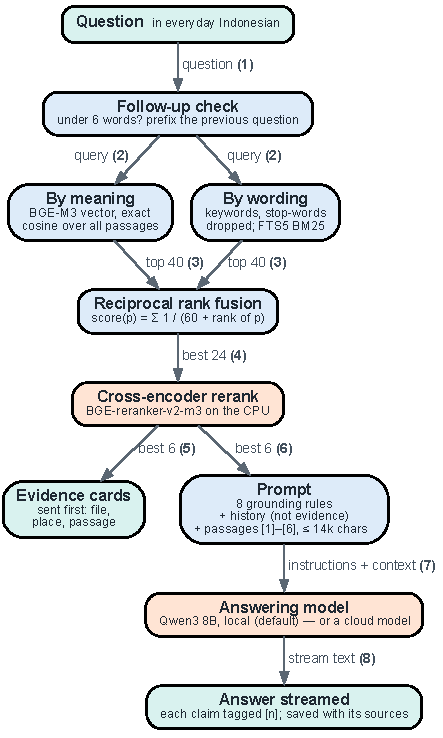
\includegraphics[width=0.8\columnwidth]{query}
\caption{Answering pipeline, with steps numbered as explained in
Section~\ref{sec:answering}; arrows sharing a number run side by side.}
\label{fig:query}
\end{figure}

Fig.~\ref{fig:query} follows a question from the input box to the screen; the
step numbers in this section refer to its arrows.

\subsubsection{Follow-up questions}
The question (step~1) first passes a follow-up check. A short follow-up such
as ``who are they?'' carries almost nothing to search for, so a question of
fewer than six words asked inside a conversation is searched together with the
previous question, which restores its subject. Longer questions are searched as
they stand, so that an unrelated earlier topic does not dilute them. The
resulting query goes to two searches at once (step~2).

\subsubsection{Two kinds of search}
\emph{Search by meaning} encodes the question with BGE-M3 and compares it with
every stored vector. This understands that ``lecturer teaching load'' and the
Indonesian abbreviation \emph{EWMP} mean the same thing though they share no
words, but it is unreliable with exact identifiers. \emph{Search by wording}
removes common Indonesian and English function words, keeps words of three
letters or more, and ranks passages with BM25 through FTS5. It finds a decree
number such as \texttt{SK-045/XYZ/VI/2025} precisely, and is blind to
paraphrase. Accreditation documents are full of both---narrative argument on one
page, decree and registration numbers on the next---so dropping either method
would quietly make a whole class of questions unanswerable. Each search returns
its 40 best passages (step~3).

\subsubsection{Fusing the rankings}
The two candidate lists cannot simply be added, because cosine similarity and
BM25 scores live on different scales. They are merged by \emph{position}
instead, with reciprocal rank fusion~\cite{rrf}:
\begin{equation}
\mathrm{score}(p) = \sum_{r \in \{\text{meaning},\,\text{wording}\}}
  \frac{1}{k + \mathrm{rank}_r(p)}, \qquad k = 60,
\end{equation}
where a passage absent from a list contributes nothing for it. A passage ranked
highly by both methods thus rises above one that only a single method
favours, and the rule needs no retuning when the collection changes. The
evidence card shows which method found each passage, which helps when
diagnosing a poor answer.

\subsubsection{Re-scoring}
The 24 best fused passages (step~4) are read once more, in full and together
with the question, by BGE-reranker-v2-m3, a cross-encoder~\cite{nogueira}, and
the six it scores highest are kept and numbered [1]--[6]. These six go both to
the browser, as evidence cards (step~5), and into the prompt (step~6). If the
reranker is
unavailable, the fused order is used instead, so the system degrades rather
than stops.

\subsubsection{Writing the answer}
The prompt has three parts. A fixed system instruction, in Indonesian, sets
eight rules, chief among them: answer only from the supplied passages; tag every
factual statement with the number of its passage; say plainly when the answer
is not there; quote numbers, names and decree numbers exactly; and point out
sources that disagree instead of silently choosing one.
Next come the last two exchanges of the conversation, at most 2{,}500
characters, explicitly labelled as context for understanding the question and
\emph{not} as evidence---otherwise a mistake in one answer could be cited as
fact two answers later. Last come the six numbered passages, each with its
document name and location, capped at 14{,}000 characters in total so they
always fit the model's 8{,}192-token context. The prompt goes to the answering
model (step~7), whose text is streamed to the browser as it is written
(step~8). The local model runs at a low temperature (0.2), with its separate
reasoning mode switched off.

Keeping to six passages follows the evidence that models use long inputs unevenly~\cite{liu}, and it
leaves room on a small graphics card. If nothing is found, the model is not
called at all, and the user is told so with suggestions for rephrasing.

\subsubsection{Choosing the model}
\label{sec:models}
The answering model is interchangeable per question, and the choice is a privacy
decision more than a technical one (Table~\ref{tab:models}). The default, Qwen3
8B, runs locally, so no document text leaves the building (R3). For harder
questions the user may select Claude, GPT or Gemini, which synthesise better
but send the six retrieved passages to their provider. These are driven through
each vendor's command-line tool, already signed in on the workstation, so no
API keys are stored; each tool runs non-interactively with its
file and shell tools disabled, so the model answers purely from the prompt and
cannot browse the archive itself. The interface states the trade-off on the
model selector, so the choice is made knowingly.

\begin{table}[t]
\caption{Models, where they run, and what leaves the building}
\label{tab:models}
\centering
\footnotesize
\begin{tabular}{@{}llll@{}}
\toprule
Role & Model & Runs on & Memory \\
\midrule
Embedding  & BGE-M3              & GPU & 1.2\,GB \\
Re-scoring & BGE-reranker-v2-m3  & CPU & 1.1\,GB \\
Answering  & Qwen3 8B, 4-bit (default) & GPU & 5.0\,GB \\
Answering  & Claude, GPT or Gemini      & cloud & --- \\
\bottomrule
\end{tabular}

\smallskip
\parbox{\columnwidth}{\scriptsize Only the last row sends text off the
premises: the question and the six retrieved passages.}
\end{table}

%% ===========================================================================
\section{Delivering Answers Reliably}
\label{sec:delivery}

The answer reaches the browser as a stream of Server-Sent Events, evidence
cards first, so the reader can start checking sources while the model---the
slowest part of a request---is still writing.

\begin{figure}[t]
\centering
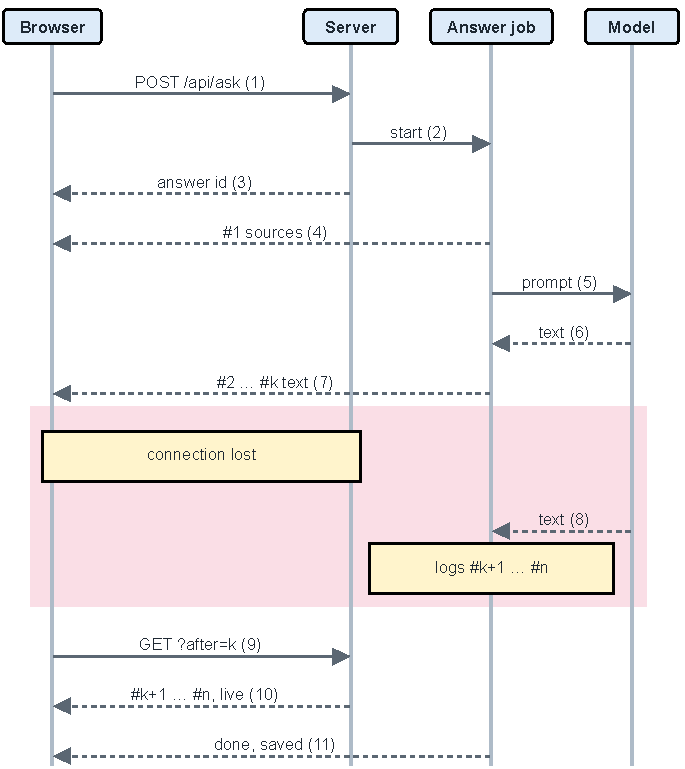
\includegraphics[width=\columnwidth]{streaming}
\caption{A resumable answer, with steps numbered as explained in
Section~\ref{sec:delivery}; \#$n$ numbers the events in the job's log.}
\label{fig:stream}
\end{figure}

Phones made a second design necessary (Fig.~\ref{fig:stream}). A local model may need most of a minute
to load after a restart, and a cloud model at its highest reasoning setting can
think for a minute before its first word; locking the screen or switching apps
in that silence drops the connection. When answers were generated inside the
HTTP response, a dropped connection killed the answer, which was then never
saved. Each question now becomes an \emph{answer job} running in its own thread
on the server, independent of any connection, which numbers and keeps every
event it produces; the HTTP response is merely a reader of that log. The step
numbers below refer to Fig.~\ref{fig:stream}. The browser posts the question
(step~1); the server starts the job (step~2) and at once returns its
identifier (step~3). The job sends the evidence cards as event \#1 (step~4),
prompts the model (step~5) and relays its text as it arrives (steps 6--7). If
the connection drops, the job carries on, logging the text that keeps arriving
(step~8). A browser that has lost its connection, heard nothing for 35 seconds,
or returned to the page after more than 15 seconds hidden asks for the events
after the last one it received, $k$ (step~9); it is sent those it missed and
then follows the live stream (step~10), until the job reports that the answer
is done and saved (step~11)---with its sources, even if nobody was watching.
The server sends a keep-alive comment every 10 seconds of silence so that idle
connections are not cut, finished jobs are kept for 30 minutes, and a Stop
button cancels the job explicitly, since closing the connection no longer
does.

%% ===========================================================================
\section{Fitting One Workstation}
\label{sec:workstation}

The deployment machine is a desktop with a 20-core Core i7-14700F, 32\,GB of
memory and an RTX~4060 graphics card with 8\,GB of video memory (R4).

\emph{Memory.} Loading all three models onto the graphics card would take about
7.3\,GB before any working memory for the model's context, risking an
out-of-memory failure in the middle of an answer, when a user is already
waiting. The re-scoring model therefore runs on the processor, where scoring two
dozen passages takes one to two seconds. Qwen3 8B is the largest model that fits
\emph{entirely} on the card with room for a long RAG context; a 14-billion
parameter model at the same precision needs about 9\,GB, spills onto the
processor, and in our trials answered at roughly a fifth of the speed.

\emph{No vector database.} The index is a SQLite file and a NumPy matrix rather
than a dedicated vector database. All 22{,}944 vectors occupy 94\,MB of memory,
and comparing a question against every one of them takes about 8\,ms on this
machine---exact, with no recall lost to approximation---while a keyword search
takes about 4\,ms. An approximate index would add a dependency and lose
recall to save time no user could notice.

\emph{Source files are never modified} (R2). The rule is enforced in software,
not by convention. Every read of a source file goes through a guard that
refuses any mode permitting writing; every write the system makes goes through a
second check that resolves symbolic links and ``..'' segments and refuses any
path inside the archive; Excel files are opened in a read-only streaming mode;
and the server refuses to start if its own data folder lies inside the archive.
Sixteen tests cover these guarantees, one of which runs a full indexing pass and
verifies that every source file is byte-for-byte unchanged. The whole suite of
481 unit tests runs in about 15 seconds without network access or model
downloads, with the models replaced by stand-ins.

%% ===========================================================================
\section{Deployment}

The system is in use for the programme's accreditation submission. Its index
covers the 1{,}497 files of Table~\ref{tab:corpus}---25.5 million characters
of text in 22{,}944 passages averaging 356 tokens---and occupies 183\,MB on
disk; the downloaded models account for most of the remaining space. During
extraction 1{,}306 pages were recognised as scans and 305 of them were
recovered by OCR. One workstation serves the whole team over the office
network, desktops and phones alike. With the local model an answer takes from a
few seconds to under a minute, depending mostly on its length; cloud models at
their highest reasoning setting typically take 30 to 60 seconds.

%% ===========================================================================
\section{Limitations and Lessons}
\label{sec:limits}

\emph{No formal evaluation yet.} We have not measured retrieval recall, answer
correctness or citation precision against a labelled set of questions. The
natural next step is to draw a few hundred questions from the accreditation
instrument, mark the passages that answer each, and measure every retrieval
stage separately alongside citation quality~\cite{alce}. The checkability of
each answer (R1) mitigates, but does not replace, such a study.

\emph{Other limits.} Legacy \texttt{.doc} and \texttt{.xls} files are not read;
OCR misreads digits on poor scans; web snapshots go stale until refreshed; the
local 8B model is noticeably weaker than cloud models at combining evidence
spread over several documents; and two shared accounts mean there is no record
of who asked what, so the guest password must be shared only within the team.

\emph{Lessons.} Remembering where every passage came from costs almost nothing,
and is what makes answers checkable. Search by meaning alone was not enough for
a corpus dense with identifiers. A network drive's failure modes look like
legitimate deletions. And the slowest step of a request should never be tied to
a single connection.

%% ===========================================================================
\section{Conclusion}

An accreditation team can have a question-answering assistant whose answers are
\emph{checkable by construction}---built from its own documents, citing them by
page, sheet or slide, leaving them untouched, and running on hardware the
department already owns. None of its components is new; the value lies in how
they are fitted to an audited, confidential and constantly changing archive. The
approach transfers to any organisation that must justify claims from a large,
messy, authoritative collection of documents.

%% ===========================================================================
\begin{thebibliography}{14}
\footnotesize

\bibitem{ji}
Z. Ji \emph{et al.}, ``Survey of hallucination in natural language
generation,'' \emph{ACM Comput. Surv.}, vol. 55, no. 12, art. 248, 2023.
[Online]. Available: \url{https://doi.org/10.1145/3571730}

\bibitem{lewis}
P. Lewis \emph{et al.}, ``Retrieval-augmented generation for knowledge-intensive
NLP tasks,'' in \emph{Proc. NeurIPS}, 2020, pp. 9459--9474. [Online]. Available:
\url{https://arxiv.org/abs/2005.11401}

\bibitem{gaosurvey}
Y. Gao \emph{et al.}, ``Retrieval-augmented generation for large language
models: A survey,'' arXiv:2312.10997, 2023. [Online]. Available:
\url{https://arxiv.org/abs/2312.10997}

\bibitem{alce}
T. Gao, H. Yen, J. Yu, and D. Chen, ``Enabling large language models to
generate text with citations,'' in \emph{Proc. EMNLP}, 2023, pp. 6465--6488.
[Online]. Available: \url{https://arxiv.org/abs/2305.14627}

\bibitem{bm25}
S. Robertson and H. Zaragoza, ``The probabilistic relevance framework: BM25 and
beyond,'' \emph{Found. Trends Inf. Retr.}, vol. 3, no. 4, pp. 333--389, 2009.
[Online]. Available: \url{https://doi.org/10.1561/1500000019}

\bibitem{dpr}
V. Karpukhin \emph{et al.}, ``Dense passage retrieval for open-domain question
answering,'' in \emph{Proc. EMNLP}, 2020, pp. 6769--6781. [Online]. Available:
\url{https://doi.org/10.18653/v1/2020.emnlp-main.550}

\bibitem{beir}
N. Thakur, N. Reimers, A. R\"uckl\'e, A. Srivastava, and I. Gurevych, ``BEIR: A
heterogeneous benchmark for zero-shot evaluation of information retrieval
models,'' in \emph{Proc. NeurIPS Datasets and Benchmarks Track}, 2021.
[Online]. Available: \url{https://arxiv.org/abs/2104.08663}

\bibitem{rrf}
G. V. Cormack, C. L. A. Clarke, and S. Buettcher, ``Reciprocal rank fusion
outperforms Condorcet and individual rank learning methods,'' in \emph{Proc.
32nd ACM SIGIR Conf.}, 2009, pp. 758--759. [Online]. Available:
\url{https://doi.org/10.1145/1571941.1572114}

\bibitem{nogueira}
R. Nogueira and K. Cho, ``Passage re-ranking with BERT,'' arXiv:1901.04085,
2019. [Online]. Available: \url{https://arxiv.org/abs/1901.04085}

\bibitem{liu}
N. F. Liu \emph{et al.}, ``Lost in the middle: How language models use long
contexts,'' \emph{Trans. Assoc. Comput. Linguist.}, vol. 12, pp. 157--173,
2024. [Online]. Available: \url{https://doi.org/10.1162/tacl_a_00638}

\bibitem{bge}
J. Chen, S. Xiao, P. Zhang, K. Luo, D. Lian, and Z. Liu, ``M3-Embedding:
Multi-linguality, multi-functionality, multi-granularity text embeddings through
self-knowledge distillation,'' arXiv:2402.03216, 2024. [Online]. Available:
\url{https://arxiv.org/abs/2402.03216}

\bibitem{qwen}
A. Yang \emph{et al.} (Qwen Team), ``Qwen3 technical report,'' arXiv:2505.09388,
2025. [Online]. Available: \url{https://arxiv.org/abs/2505.09388}

\bibitem{fts5}
SQLite Consortium, ``SQLite FTS5 extension.'' [Online]. Available:
\url{https://www.sqlite.org/fts5.html}

\end{thebibliography}

\end{document}
